\chapter{Követelmények a játékommal szemben}
\indent \indent Játék tervezésénél fontos szem előtt tartani azokat a követelményeket, amelyeknek meg kell felelnie. A felhasználói élmény szorosan kapcsolódik ahhoz, hogy a játékosok mennyire értik meg a játék működését, és ezen élmény tervezése alapvető fontosságú.


\section{Felhasználói élmény kialakítása}

\indent \indent A felhasználói élmény kialakítása során kiemelt figyelmet kell fordítani az elrendezésre, az egyértelmű utasításokra. A játékosoknak világosan kell látniuk, hogy hogyan tudnak interakcióba lépni a játék világával, és ezek az elemek nagyban hozzájárulnak a felhasználói élmény minőségéhez.

Az érthető és könnyen kezelhető felhasználói felület kulcsfontosságú a játék sikeréhez. A játékosoknak könnyen kell tudniuk kezelni a játék funkcióit és lehetőségeit, hogy maximálisan élvezhessék a játékot.

Az is fontos tényező, hogy a játék érthetősége és használhatósága ne csak a tapasztalt játékosok számára legyen megfelelő, hanem a kezdők és a kevésbé jártas személyek számára is könnyen hozzáférhető legyen. Az egyszerű és intuitív felület tervezése segíthet abban, hogy minél több játékos élvezhesse a játékot.


\section{Grafika}

\indent \indent A játékok szempontjából a grafika kulcsfontosságú elem. Egy gondosan kidolgozott vizuális megjelenés mélyebben bevonja a játékosokat a játék világába, ami növeli a játék élvezetét.

Ezért fontos számomra, hogy saját magam készítsem el a rajzokat, ezzel is egyedivé téve a játékot, illetve a fejlesztés során egyszerűbben áthidalhatóak a grafikai problémák, hiszen nem kell harmadik féllel egyeztetnem. A pálya kirajzolásánál szeretnék megvalósítani hamis 3D-s hatást, hogy a játékosok számára élethűbbnek tűnjön a játék. 


\section{Menürendszer}

\indent \indent A menürendszernek általában a játékhoz illőnek kell lennie, hogy a játékosok ne érezzék azt, hogy egy másik játékot indítanak el. Fontos az is, hogy átlátható legyen, hogy a játékosok könnyen eligazodjanak benne, és ne kelljen sok időt tölteniük azzal, hogy megtalálják a keresett funkciót. (Lásd \ref{fig:Menürendszer terve} ábra)

\begin{figure}[H]
    \centering
    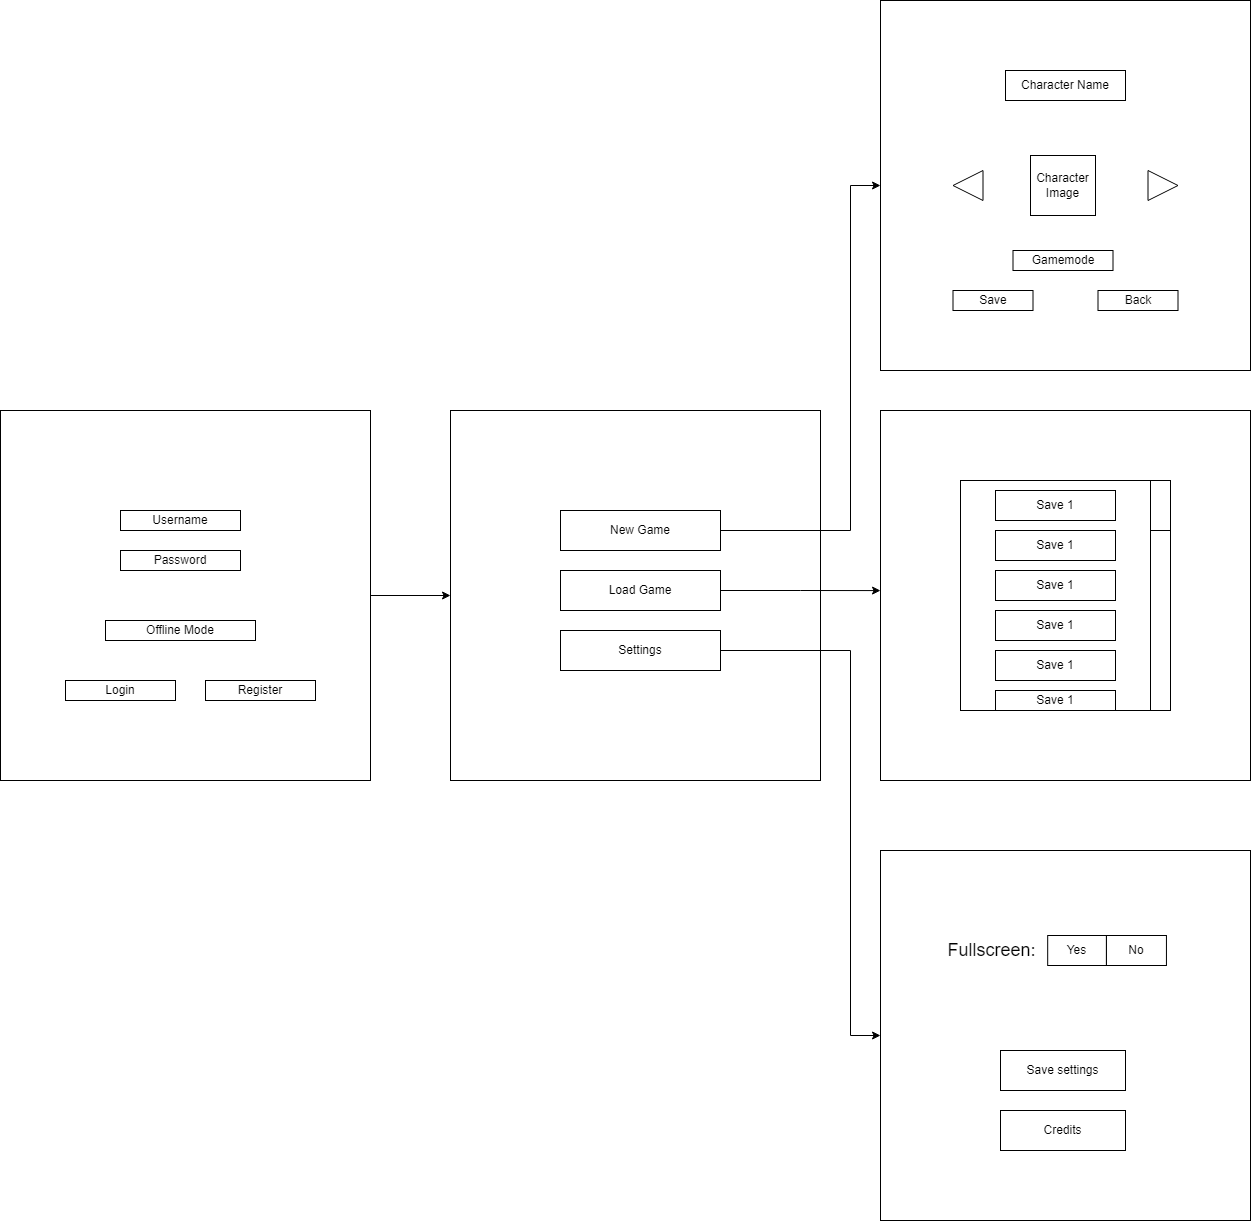
\includegraphics[width=14.0truecm]{images/MS_menu.drawio.png}
    \caption{Menürendszer terve}
    \label{fig:Menürendszer terve}
\end{figure}

\subsection{Felhasználói fiók}
\indent \indent Felhasználói fiókok létrehozása azért volt szükséges a játékomban, mivel szerettem volna létrehozni egy ranglista rendszert, ahol a játékosok tudhatták, hogy egymással versenyeznek, hogy ki hányszor vitte végig a játékot anélkül, hogy a karakterük egyszer is meghalt volna, miközben a szörnyek minden újrakezdés után erősödtek. Ehhez a rendszerhez elengedhetetlen volt, hogy meg tudjam különböztetni a játékosokat, illetve, hogy egy adatbázisban tudjam tárolni a játékosok adatait. (Lásd \ref{fig:Relációs modell} ábra)

\begin{figure}[t]
    \centering
    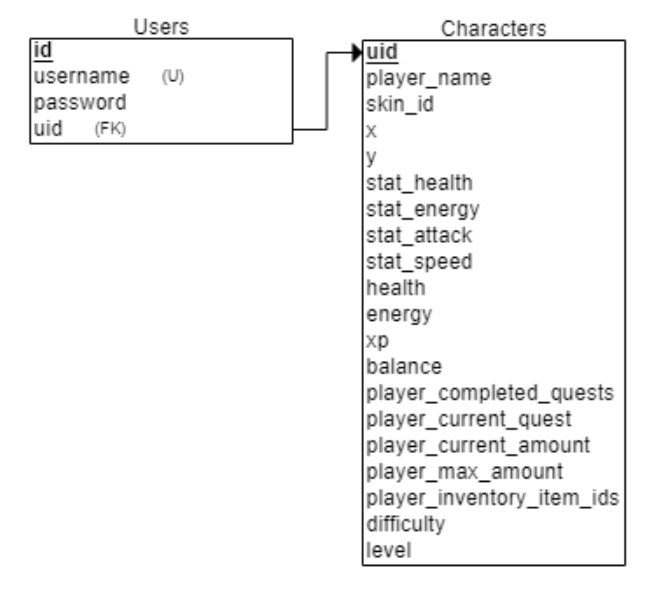
\includegraphics[width=10.0truecm]{images/RelationModell.png}
    \caption{Relációs modell}
    \label{fig:Relációs modell}
\end{figure}

\subsection{Főmenü funkciói}

\indent \indent A bejelentkezést követően három menüpont válik elérhetővé a játékosok számára. Az egyik kiemelkedően fontos lehetőség a beállítások menüpont, mivel általában itt találhatók a kulcsfontosságú funkciók módosítására szolgáló lehetőségek. Az én esetemben itt érhető el a teljes képernyős mód beállítása. A beállítások menüpont alatt továbbá megtalálható egy "Credits" opció is, ami tartalmazza a készítő nevét és az elkészítés évét. A másik két menüpont a játék indításával kapcsolatos: lehetőség van új karakter létrehozására, illetve meglévő mentéseik betöltésére.

\subsection{Játékon belüli menürendszer}

\indent \indent A legtöbb játékban kiemelkedő jelentőségű a játékon belüli pillanat állj funkció, és egy ilyenkor megjelenő belső menürendszer. Lényeges, hogy ezek könnyen elérhetőek legyenek, miközben nem zavarják a játékélményt. A játékosoknak lehetőségük van a játék közben is hozzáférni egy beállítások menühöz, amelyben a hangerőszintet is be tudják állítani. Ezen menü részét kell képeznie egy mentés funkciónak, ami a játék aktuális állapotának mentését teszi lehetővé, továbbá egy folytatás lehetőségnek, és egy kilépés opciónak, amely a játék bezárását szolgálja.


\section{Felhasználói felület és a játékos cselekvési lehetőségei}

\indent \indent A játékokban fontos a jól megtervezett felhasználói felület amit a játék közben lát a játékos, amely lehetővé teszi a játékosok számára, hogy a lehető legkönyebben és leggyorsabban elérjék a kívánt funkciókat. Ilyen felület a HUD (Head Up Display), amely segíti a játékosokat abban, hogy valós idejű információkkal rendelkezzenek a játék világáról és saját karakterük aktuális állapotáról, így gyorsabban és hatékonyabban reagálhatnak a különböző helyzetekre.


\subsection{Felhasználói felület}

\indent \indent A felhasználói felület megtervezése során, nagyon kell figyelni a letisztultságra és a felhasználói élményre. Fontosnak tartottam, hogy a design egyszerű és könnyen átlátható legyen, hogy a felhasználó könnyedén megtalálja azokat a funkciókat és információkat, amelyekre szüksége van.

A Head Up Display (HUD) a játékos karakterének életpontjait, energia szintjét, a játékos aranyát, a játékos szintjét, a játékos tapasztalati pontjait, a játékos fegyverét, a játékos által használt italokat fogja megjeleníteni.
A HUD a játék során folyamatosan látható lesz, így a játékosoknak nem kell külön menübe navigálniuk, hogy megtalálják a folyamatosan szükséges és releváns információkat és cselekvési lehetőségeket. (Lásd \ref{fig:Felhasználói felület} ábra)

\begin{figure}[H]
    \centering
    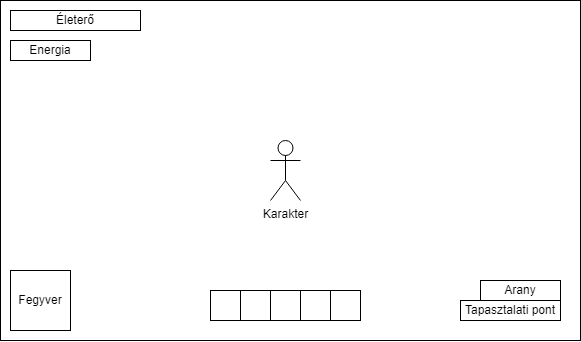
\includegraphics[width=14.0truecm]{images/MS_UI.drawio.png}
    \caption{Felhasználói felület terve}
    \label{fig:Felhasználói felület}
\end{figure}

\subsection{Életpontok és energia}

\indent \indent A játékos karakterének életpontjai mutatják meg, hogy mennyi sebzést tudnak még elviselni, mielőtt meghalna a karakterük. Az energia szint pedig a karakter futásához és cselekvéseihez szükséges energiaforrás. A megfelelő kezelése és felhasználása kulcsfontosságú a túléléshez és a harc hatékonyságához.

\subsection{Fegyverválasztás}

\indent \indent A játékosnak lehetősége van választani számos közelharci fegyver közül, amelyeket a preferenciája alapján szabadon választhat meg. A fegyverek különböző sebzést okoznak, de ez függ a hatótávolságuktól is. Hiszen a rövidebb hatótávolságú fegyverekkel közelebb kell kerülni az ellenségekhez, hogy sebzést okozzon a játékos, ez nagyobb kockázattal jár ezért azokkal több sebzést lehet okozni.

\subsection{Harcolás szörnyekkel}

\indent \indent A játék során a játékosnak számos szörnnyel kell megküzdenie. A harcok izgalmasak és változatosak, például a varázsló tud a pálcájából lövedékeket lőni a karakter irányába, amelyeket olykor nehéz kikerülni. A játékosnak ki kell használnia a karaktere képességeit és fegyvereit a sikeres küzdelem érdekében. A szörnyek legyőzése tapasztalati pontokat (XP) és esetleges zsákmányt is eredményez.

\subsection{Küldetések felvétele}

\indent \indent A lineáris történetvezetés lehetőséget kínál arra, hogy a játékosok fokozatosan merüljenek el a játék világában, miközben követik a fő cselekményt. A küldetések integrálása a lineáris narratívába lehetővé teszi, hogy a játékosok szorosan kövessék a történet fő vonalát, miközben változatos kihívásokkal találkoznak.

A küldetések kiváló lehetőséget nyújtanak a karakterfejlődésre és a történet gazdagítására. Az XP (tapasztalati pont) és jutalmak rendszere ösztönzi a játékosokat, hogy aktívan részt vegyenek a küldetésekben, és ezáltal fokozatosan erősödjenek a játékban. A lineáris elbeszélésmód segítségével a küldetések sorrendje és nehézségi szintje könnyen szabályozható, így biztosítható a folyamatos kihívás és az érdekesség fenntartása.

\subsection{Bájitalok vásárlása és használata}

\indent \indent A játékos aranyat szerezhet a játék során, amit bájitalokra is fordíthat. Azokat különböző hatásokkal rendelkeznek, például sebzés gyógyítása vagy energiaszint növelése. A bájitalok stratégiai használata a túlélés és a harcok kulcsa lehet.

\subsection{Statisztikák növelése tapasztalati pontokból}

\indent \indent A játékos karaktere tapasztalati pontokat szerez a harcok és küldetések során. Az XP felhasználható a karakter statisztikáinak növelésére, például az erő, az ügyesség vagy a mágia terén. Ez lehetővé teszi a karakter fejlődését, specializálását és ezzel a játékmenet testreszabását.

Ezen cselekvési lehetőségek összekapcsolva teremtenek egy gazdag és dinamikus játékélményt az Action RPG (akció-szerepjátékban) játékban, ahol a játékos döntései és cselekedetei hatással vannak a karakter fejlődésére és a játék világára.



